%=====================================================================
%  SRRT --- IEEE conference paper (IEEEtran), 6 pages
%
%  Compile:  pdflatex srrt_ieee && pdflatex srrt_ieee
%  Requires: IEEEtran.cls (TeX Live / MiKTeX / Overleaf "IEEE Conference")
%            figures in paper/figures/*.pdf, produced by
%            scripts/make_paper_figures.py
%
%  EXPERIMENTAL RECORD
%  -------------------
%  All six configurations trained 60 epochs, cosine T_max=60 annealed to
%  eta_min, evaluated on 1111 GoPro test images. Every number below is
%  measured. Provenance for each figure is in paper/figures/*.json.
%=====================================================================
\documentclass[conference]{IEEEtran}
\IEEEoverridecommandlockouts

\usepackage{cite}
\usepackage{amsmath,amssymb,amsfonts}
\usepackage{graphicx}
\usepackage{textcomp}
\usepackage{xcolor}
\usepackage{booktabs}
\usepackage{tikz}
\usetikzlibrary{arrows.meta,positioning,calc,fit,backgrounds}

% Search both a figures/ subfolder and the main directory, so the paper builds
% whether the figures are uploaded into a folder or flat alongside the .tex.
\graphicspath{{figures/}{./}{../figures/}}

% Compact floats so six pages actually hold six pages of content.
\setlength{\textfloatsep}{7pt plus 2pt minus 2pt}
\setlength{\floatsep}{7pt plus 2pt minus 2pt}
\setlength{\intextsep}{7pt plus 2pt minus 2pt}
\setlength{\abovecaptionskip}{3pt}

\newcommand{\bs}[1]{\textbf{#1}}

\begin{document}

\title{Semantic Rectified Restoration Transformer:\\
Zero-Gated Latent Guidance for Image Deblurring}

\author{\IEEEauthorblockN{Author One}
\IEEEauthorblockA{\textit{Dept. of Computer Science and Engineering} \\
\textit{Institution Name}\\
City, Country \\
email@domain}
\and
\IEEEauthorblockN{Author Two}
\IEEEauthorblockA{\textit{Dept. of Computer Science and Engineering} \\
\textit{Institution Name}\\
City, Country \\
email@domain}
}

\maketitle

%=====================================================================
\begin{abstract}
Transformer backbones such as Restormer restore images from low-level evidence
alone, carrying no explicit representation of \emph{what} is being
reconstructed. We present the Semantic Rectified Restoration Transformer
(SRRT), which augments a Restormer backbone with a semantic latent pathway: a
visual context encoder, a damage-aware encoder, a latent consistency
regularizer (LCR), a rectified-flow latent transport, and a semantic refinement
attention block (SRA). Every module joins at the bottleneck through a
\emph{zero-initialized gate}, so untrained SRRT is bitwise identical to the
backbone it extends and each rung of the ablation ladder begins from the same
function. We train all six cumulative configurations to convergence under an
identical 60-epoch schedule and evaluate on 1111 GoPro test images. Rectified
flow gives the largest gain, $+0.122$~dB PSNR over the baseline (95\% CI
$[+0.102,+0.142]$, winning on 756 of 1111 images); LCR contributes $+0.077$~dB
and the best LPIPS; the damage-aware encoder is statistically
indistinguishable from baseline; and SRA, the final module, \emph{removes} the
accumulated gain entirely. We additionally report two methodological findings.
A zero-output equivalence test cannot establish that a module is integrated---a
gated module and a module wired to nothing are indistinguishable under it---and
a complementary gradient-flow test caught a real defect in our implementation.
Separately, an auxiliary objective whose regression target is produced by a
shared trainable encoder admits a degenerate solution; ours reduced its loss
$31\times$ by corrupting the restoration encoder, costing 10~dB, until the
target was detached. Effects are small and each arm is a single training run,
so we report per-image confidence intervals and state plainly what they do and
do not license.
\end{abstract}

\begin{IEEEkeywords}
image restoration, motion deblurring, vision transformer, semantic guidance,
rectified flow, ablation methodology, reproducibility
\end{IEEEkeywords}

%=====================================================================
\section{Introduction}

Single-image motion deblurring recovers a sharp image $\hat{x}$ from a blurred
observation $y$. Transformer architectures---Restormer~\cite{restormer},
SwinIR~\cite{swinir}, Uformer~\cite{uformer}---dominate the task, modelling
long-range dependencies while remaining tractable at high resolution.

They share a limitation. Trained end-to-end on pixel and perceptual
reconstruction objectives, they learn a mapping driven entirely by low-level
appearance statistics, with no explicit representation of scene content and
none of how the image was degraded. When blur is severe the problem is
ill-posed: many sharp images explain the observation, and a purely
appearance-driven prior has little basis for choosing among them.

This paper asks whether an explicit semantic latent pathway helps, and designs
the study so the contribution of each module is measurable in isolation. Our
contributions are:

\begin{enumerate}
\item \bs{A modular semantic restoration architecture.} SRRT couples a
Restormer backbone to a semantic pathway of five modules operating on the
bottleneck latent (Section~\ref{sec:method}).

\item \bs{Zero-gated integration.} Every module joins through a
zero-initialized additive gate, making untrained SRRT \emph{bitwise} identical
to Restormer. Any measured difference is therefore attributable to what a
module learned, not to a perturbation it introduced at initialization.

\item \bs{A complete, converged ablation ladder.} All six configurations are
trained under an identical schedule and compared per-image with confidence
intervals and signed-rank tests (Section~\ref{sec:results}). Rectified flow
helps most; SRA cancels the gain.

\item \bs{Two transferable methodological findings:} that equivalence testing
cannot verify integration, and that an auxiliary loss with a trainable target
is degenerate by construction (Sections~\ref{sec:connectivity},
\ref{sec:flowfailure}).
\end{enumerate}

%=====================================================================
\section{Related Work}

\bs{Transformer restoration.} Restormer~\cite{restormer} replaces spatial
self-attention with multi-Dconv head transposed attention, computing attention
across \emph{channels} (Section~\ref{sec:method}). SwinIR~\cite{swinir} and
Uformer~\cite{uformer} instead use shifted local windows, and
NAFNet~\cite{nafnet} argues much of the gain is architectural simplification
rather than attention.

\bs{Semantic and degradation priors.} Semantic priors condition restoration
through segmentation maps or CLIP-style embeddings. SeeCoder~\cite{seecoder},
built for prompt-free diffusion, encodes an image into dense visual context
intended to replace a text prompt; we adopt it as content-level context.
Diffusion autoencoders~\cite{diffae} learn a decodable semantic latent; we
reuse the encoder design not to generate but to produce a \emph{damage-aware}
representation. No disentanglement is guaranteed---it is a learned
representation and nothing more, a caveat Section~\ref{sec:results} finds
warranted.

\bs{Flow transport.} Rectified flow~\cite{rectifiedflow} learns a velocity
field transporting one distribution to another along near-straight paths,
permitting few-step integration. We apply it in latent space, between a
degraded-image and a clean-image latent.

%=====================================================================
\section{Proposed Method}
\label{sec:method}

\begin{figure}[t]
\centering
\scriptsize
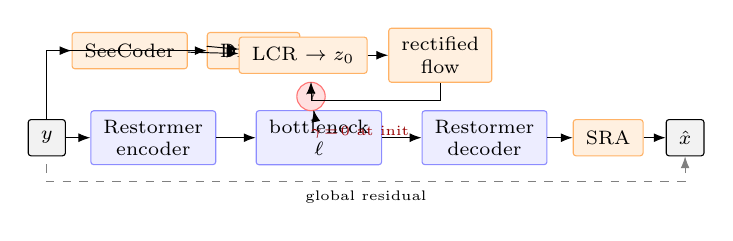
\begin{tikzpicture}[
  node distance=3.1mm,
  box/.style={draw, rounded corners=1pt, minimum height=4.6mm, align=center,
              inner xsep=1.6mm, font=\scriptsize},
  bb/.style ={box, fill=blue!7,   draw=blue!45},
  sem/.style={box, fill=orange!12, draw=orange!60},
  gate/.style={draw, circle, inner sep=0.4pt, font=\tiny, fill=red!12,
               draw=red!55, minimum size=3.6mm},
  fl/.style={-{Latex[length=1.5mm]}, line width=0.35pt},
]
\node[box, fill=gray!10] (y) {$y$};
\node[bb, right=of y] (enc) {Restormer\\encoder};
\node[bb, right=5.0mm of enc] (bn) {bottleneck\\$\ell$};
\node[bb, right=5.0mm of bn] (dec) {Restormer\\decoder};
\node[sem, right=3.2mm of dec] (sra) {SRA};
\node[box, fill=gray!10, right=2.8mm of sra] (xh) {$\hat{x}$};

\node[sem, above=5.2mm of enc, xshift=-3mm] (see) {SeeCoder};
\node[sem, right=2.4mm of see] (dae) {DiffAE};
\node[sem, above=4.6mm of bn, xshift=-2mm] (lcr) {LCR $\rightarrow z_0$};
\node[sem, right=2.6mm of lcr] (rf) {rectified\\flow};

\node[gate] (g1) at ($(bn)!0.5!(lcr)$) {$\gamma$};

\draw[fl] (y) -- (enc);
\draw[fl] (enc) -- (bn);
\draw[fl] (bn) -- (dec);
\draw[fl] (dec) -- (sra);
\draw[fl] (sra) -- (xh);

\draw[fl] (y.north) |- (see.west);
\draw[fl] (y.north) |- (dae.west);
\draw[fl] (see) -- (lcr);
\draw[fl] (dae) -- (lcr);
\draw[fl] (lcr) -- (rf);
\draw[fl] (rf.south) -- ++(0,-2.2mm) -| (g1.north);
\draw[fl] (g1) -- (bn);

\draw[fl, dashed, gray] (y.south) ++(0,-1mm) -- ++(0,-2.2mm) -|
   node[pos=0.25, below, font=\tiny, black] {global residual} (xh.south);

\node[font=\tiny, red!60!black, below=0.6mm of g1, xshift=6.2mm]
  {$\gamma\!=\!0$ at init};
\end{tikzpicture}
\caption{SRRT. The Restormer path (blue) is untouched. The semantic pathway
(orange) meets it at the bottleneck through a gate $\gamma$ initialized to
exactly zero, so at initialization $\mathrm{SRRT}(y)=\mathrm{Restormer}(y)$
bitwise for every configuration.}
\label{fig:arch}
\end{figure}

\subsection{Problem formulation}
Let $x\in\mathbb{R}^{3\times H\times W}$ be the unknown clean image and
$y\in\mathbb{R}^{3\times H\times W}$ the degraded observation. Restoration is
the inverse problem
\begin{equation}
y = \mathcal{D}(x) + n,
\label{eq:inverse}
\end{equation}
with $\mathcal{D}$ a degradation operator and $n$ noise. For motion blur
$\mathcal{D}$ is a convolution, $y = k * x + n$, with $k$ the blur kernel. The
map $y\mapsto x$ is ill-posed: distinct clean images can yield near-identical
observations, $\mathcal{D}(x_1)\approx\mathcal{D}(x_2)$, so restoration depends
on a prior rather than on inversion alone. SRRT's premise is that this prior
should include explicit representations of scene content and of the degradation
itself, not only low-level appearance statistics.

\subsection{Notation}
Table~\ref{tab:notation} fixes the symbols used throughout.

\begin{table}[t]
\caption{Notation. Backbone symbols follow Restormer~\cite{restormer}.}
\label{tab:notation}
\centering
\footnotesize
\setlength{\tabcolsep}{3.5pt}
\begin{tabular}{@{}ll@{}}
\toprule
Symbol & Meaning \\
\midrule
$x,\;y,\;\hat{x}$ & clean image, degraded observation, restoration \\
$\mathcal{D},\;n$ & degradation operator, noise \\
$X,\;X',\;Y$ & block input, post-MDTA, block output tensors \\
$B,C,H,W$ & batch, channels, feature height, width \\
$h,\;d$ & attention heads, channels per head; $C=hd$ \\
$Q,K,V$ & query, key, value tensors, $\mathbb{R}^{B\times h\times d\times HW}$ \\
$\alpha$ & learned attention scaling parameter \\
$\ell,\;\ell'$ & bottleneck latent before / after injection \\
$z_0$ & LCR-fused latent from SeeCoder and DiffAE \\
$z_1$ & latent of the clean target (detached) \\
$z_t$ & interpolated latent at time $t\in[0,1]$ \\
$v_\theta,\;v^\star$ & predicted and ideal velocity field \\
$\gamma,\;\gamma_{\text{SRA}}$ & zero-initialized gates \\
$\odot,\;\mathrm{sg}[\cdot]$ & elementwise product, stop-gradient \\
\bottomrule
\end{tabular}
\end{table}

\subsection{Overview}
SRRT keeps the Restormer encoder--bottleneck--decoder path intact and adds a
parallel semantic pathway meeting the backbone at the \emph{bottleneck}
(Fig.~\ref{fig:arch}). The bottleneck is the natural junction: it is the
lowest-resolution, most semantic tensor in the network ($8C$ channels at
$H/8\times W/8$), so latent transport is cheap there, and the decoder still has
three upsampling stages in which to propagate what the latent contributes.

Given $y \in \mathbb{R}^{3\times H\times W}$, the encoder produces skip
features and a bottleneck latent $\ell$. The semantic pathway produces a latent
$z$, injected as
\begin{equation}
\ell' = \ell + \gamma \cdot W_{\text{inj}}(z),
\label{eq:inject}
\end{equation}
where $W_{\text{inj}}$ is a $1\!\times\!1$ convolution and $\gamma$ a scalar
gate initialized to zero.

\subsection{Backbone}
We use Restormer~\cite{restormer} with $C=48$, a four-level encoder, three-level
decoder with pixel-shuffle resampling, and a refinement stage.
\emph{Equations~\eqref{eq:block1}--\eqref{eq:gdfn} are Restormer's, reproduced
here with full variable definitions because the behaviour of
Section~\ref{sec:flowfailure} depends on which tensors are shared.}

Each transformer block is two residual sub-blocks. The first applies
multi-Dconv head transposed attention to a layer-normalized input; the second
applies a gated-Dconv feed-forward network:
\begin{align}
X' &= X + \mathrm{MDTA}\big(\mathrm{LN}(X)\big), \label{eq:block1}\\
Y  &= X' + \mathrm{GDFN}\big(\mathrm{LN}(X')\big), \label{eq:block2}
\end{align}
so a block realizes $X \to \mathrm{LN} \to \mathrm{MDTA} \to X' \to
\mathrm{LN} \to \mathrm{GDFN} \to Y$. The residual additions let each block
learn a refinement rather than reconstruct its input.

\textbf{MDTA.} For $X\in\mathbb{R}^{B\times C\times H\times W}$, queries, keys
and values come from a pointwise followed by a depthwise convolution,
$Q,K,V = \mathrm{DWConv}(\mathrm{Conv}_{1\times1}(X))$, reshaped into $h$ heads
of $d=C/h$ channels. Attention is then formed \emph{across channels}:
\begin{equation}
A = \mathrm{softmax}\!\left(\hat{Q}\hat{K}^{\top}/\alpha\right), \qquad
A \in \mathbb{R}^{B\times h\times d\times d},
\label{eq:mdta}
\end{equation}
with $\hat{Q},\hat{K}$ $\ell_2$-normalized along the spatial axis and $\alpha$
a learned scale. The attention matrix is $d\!\times\!d$ over channels, never
$HW\!\times\!HW$ over positions. This is the entire efficiency argument:
conventional spatial attention costs $\mathcal{O}((HW)^2C)$ against
$\mathcal{O}(HW\,C^2)$ here, and at $H=W=256$, $C=48$ the interaction matrix is
$48^2$ rather than $65{,}536^2$ --- the latter alone being 17.2~GB in FP32.

\textbf{GDFN.} The feed-forward path gates one half of a depthwise-convolved
projection by the other:
\begin{equation}
\mathrm{GDFN}(X) = W_o\big[\mathrm{GELU}(X_a)\odot X_b\big],\quad
[X_a,X_b] = W_{dw}W_pX,
\label{eq:gdfn}
\end{equation}
where $W_p$, $W_{dw}$, $W_o$ are the pointwise, depthwise and output
projections. The depthwise convolution supplies spatial awareness inside the
feed-forward block.

Across the hierarchy, resolution halves and width doubles at each level,
$48\!\to\!96\!\to\!192\!\to\!384$ channels, giving a bottleneck latent
$\ell\in\mathbb{R}^{B\times 384\times H/8\times W/8}$ --- the tensor the
semantic pathway writes into. The network predicts a global residual,
$\hat{x}=f(y)+y$.

\subsection{Semantic modules}

\bs{SeeCoder} encodes $y$ into dense visual context at $H/8\times W/8$, width
256, via a lightweight multi-scale encoder and self-attention blocks.

\bs{DiffAE} encodes $y$ into a spatial damage latent and a pooled semantic
code, intended to capture degradation characteristics.

\bs{LCR} fuses the visual and damage latents into an initial restoration latent
$z_0$ and imposes consistency against a reference $z_{\text{ref}}$ obtained by
encoding the ground truth. Both pass through a \emph{shared} projection $g$ and
are $\ell_2$-normalized:
\begin{equation}
\mathcal{L}_{\text{cons}} = \left\|
\tfrac{g(z_0)}{\|g(z_0)\|_2} -
\tfrac{g(\mathrm{sg}[z_{\text{ref}}])}{\|g(\mathrm{sg}[z_{\text{ref}}])\|_2}
\right\|_2^2 ,
\label{eq:lcr}
\end{equation}
where $\mathrm{sg}[\cdot]$ is a stop-gradient. Normalization makes the
objective scale-invariant so it cannot be minimized by shrinking norms; the
stop-gradient prevents the reference collapsing toward the prediction.

\bs{Rectified flow}~\cite{rectifiedflow} transports $z_0$ toward the
clean-image latent $z_1$ along a straight path. Interpolating
$z_t=(1-t)z_0+tz_1$ and differentiating gives the ideal velocity directly,
\begin{equation}
\frac{dz_t}{dt} = z_1 - z_0 \;=\; v^\star ,
\label{eq:velocity}
\end{equation}
which is constant along the path --- this is what ``rectified'' refers to, and
why few integration steps suffice. The network regresses it:
\begin{equation}
\mathcal{L}_{\text{flow}} = \mathbb{E}_{t\sim\mathcal{U}(0,1)}
\left\| v_\theta(z_t,t) - (\mathrm{sg}[z_1] - z_0) \right\|_2^2 .
\label{eq:flow}
\end{equation}
Critically $z_1$ enters \emph{detached}, and the backbone is injected with
$z_0$ during training, not $z_1$; Section~\ref{sec:flowfailure} shows what
happens otherwise. At inference $z_1$ is unavailable and $\hat{z}_1$ is
recovered by 20-step Euler integration of $dz/dt=v_\theta(z,t)$ from $z_0$,
in FP32 under no-grad.

\bs{Equation provenance.} Equations~\eqref{eq:block1}--\eqref{eq:gdfn} are
Restormer's~\cite{restormer} and \eqref{eq:velocity} is the rectified-flow
construction of~\cite{rectifiedflow}. Equations~\eqref{eq:inject},
\eqref{eq:lcr}, \eqref{eq:flow} as applied here, and the SRA formulation below
are proposed in this work; they are not established methods and should not be
cited as prior art.

\bs{SRA} forms a spatial attention map $A_s$ over the refined decoder features
$F$ and uses it to weight a predicted residual correction $R(F)$, the intent
being to concentrate capacity where restoration error remains:
\begin{equation}
F' = F + \gamma_{\text{SRA}}\cdot A_s \odot R(F).
\label{eq:sra}
\end{equation}
Section~\ref{sec:results} finds this module does not deliver that intent.

\subsection{Zero-gated integration}
\label{sec:zerogatemethod}
Each module enters through a gate initialized to exactly zero: $\gamma=0$ in
\eqref{eq:inject}, $\gamma_{\text{SRA}}=0$, and the flow output projection is
zero-initialized so $v_\theta\equiv 0$ and the ODE is the identity map.

At initialization, therefore, $\mathrm{SRRT}(y)=\mathrm{Restormer}(y)$
\emph{bitwise} for every configuration. We verified this for all six: the
maximum absolute output deviation from the bare backbone is exactly $0.0$, not
merely within floating-point tolerance, since the gates are exactly zero and
the products vanish identically. This is a methodological device, not an
implementation detail---it guarantees every rung of the ladder begins from the
same function.

Gradient still reaches $\gamma$ at the first step, since
$\partial\mathcal{L}/\partial\gamma = \langle \partial\mathcal{L}/\partial\ell',
W_{\text{inj}}(z)\rangle \neq 0$, so the gate opens and the module trains from
step two onward.

\subsection{Training objective}
\begin{equation}
\mathcal{L} = \lambda_1 \mathcal{L}_{1}
            + \lambda_p \mathcal{L}_{\text{perc}}
            + \lambda_f \mathcal{L}_{\text{flow}}
            + \lambda_c \mathcal{L}_{\text{cons}},
\label{eq:total}
\end{equation}
with $\lambda_1=1.0$, $\lambda_p=0.1$ (VGG19~\cite{vgg}), $\lambda_f=0.1$,
$\lambda_c=0.1$. Flow and consistency terms are included \emph{only} when their
modules are enabled, so each rung trains under exactly the objective its
architecture implies.

%=====================================================================
\section{Experimental Setup}
\label{sec:setup}

\bs{Data.} GoPro~\cite{gopro}: 2103 train and 1111 test pairs, normalized to
$[0,1]$. Training uses $128\times128$ random crops with augmentation;
evaluation uses $256\times256$ center crops without.

\bs{Optimization.} AdamW~\cite{adamw} ($\eta=2\times10^{-4}$, weight decay
$10^{-4}$), batch size 2 with gradient accumulation 4 (effective batch 8),
gradient clipping 1.0, cosine annealing~\cite{sgdr} with $T_{\max}$ equal to
the epoch count and $\eta_{\min}=10^{-6}$, mixed precision~\cite{amp}, seed 42.
All runs use one NVIDIA RTX 4070 Laptop GPU (8~GB).

\bs{Budget.} 60 epochs, 1051 iterations per epoch, 15{,}720 optimizer steps.
Because $T_{\max}$ is tied to the epoch count, the learning rate reaches
$\eta_{\min}$ exactly when training ends. \emph{All six arms share this
schedule}; a run that stops mid-descent is not comparable to one that anneals,
and we exclude such runs rather than report them (Section~\ref{sec:admis}).

\bs{Metrics.} PSNR, SSIM~\cite{ssim}, LPIPS~\cite{lpips} (AlexNet). LPIPS is
deliberately not the training objective---training uses a VGG19 perceptual
loss---so it remains an independent measure.

\bs{Ladder.} Six cumulative configurations (Table~\ref{tab:main}), each
differing from its predecessor by exactly one module, sharing dataset,
protocol, optimizer, schedule and seed.

\subsection{Validation methodology}
\label{sec:connectivity}
Before training we require two independent checks.

\bs{Zero-gate equivalence:} each configuration's output at initialization must
equal the bare backbone's, given shared backbone weights.

\bs{Connectivity:} every enabled module must receive non-zero gradient from the
\emph{full} objective once the gate has opened.

The second is not redundant. A module behind a zero gate and a module wired to
nothing produce \emph{identical} output at initialization, and both pass the
first check with error exactly zero; they differ only after the first optimizer
step. In our implementation the SeeCoder pathway was initially constructed only
when a downstream module was also enabled, so the SeeCoder-only configuration
instantiated 335{,}380 parameters, consumed compute every forward pass, and
never received gradient. Perturbing every SeeCoder weight by
$\mathcal{N}(0,10)$ changed the output by exactly $0.0$, and $0/44$ SeeCoder
tensors had a gradient---while the zero-gate check reported a perfect pass
throughout. The general point: \emph{equivalence tests validate
initialization, not integration.}

The connectivity test must also score the full objective. With flow enabled the
backbone receives the supervised endpoint during training, so the
SeeCoder$\rightarrow$LCR$\rightarrow z_0$ path reaches the loss through
$\mathcal{L}_{\text{flow}}$ and $\mathcal{L}_{\text{cons}}$ rather than the
pixel term; a test scoring only pixel loss would report those modules
disconnected.

%=====================================================================
\begin{figure*}[t]
\centering
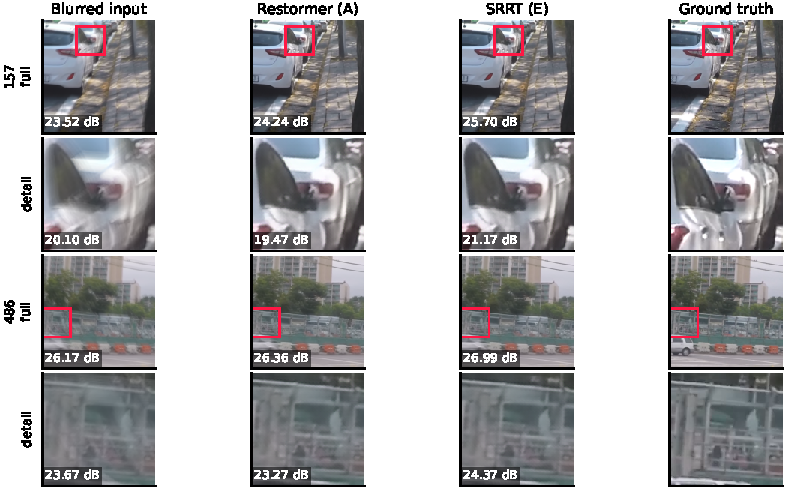
\includegraphics[width=\textwidth]{fig_qualitative.pdf}
\caption{Qualitative comparison on GoPro. For each test image the upper row
shows the full restored output with the magnified region boxed, and the lower
row the magnified detail: blurred input, Restormer baseline (A), SRRT with
rectified flow (E), and ground truth. PSNR is reported \emph{for the panel
shown} --- whole-image above, patch below. The magnified window is chosen to
maximize the baseline-minus-SRRT squared error and is therefore favourable to
SRRT by construction; the unselected full-test-set averages are those in
Table~\ref{tab:main}.}
\label{fig:qual}
\end{figure*}

\begin{figure*}[t]
\centering
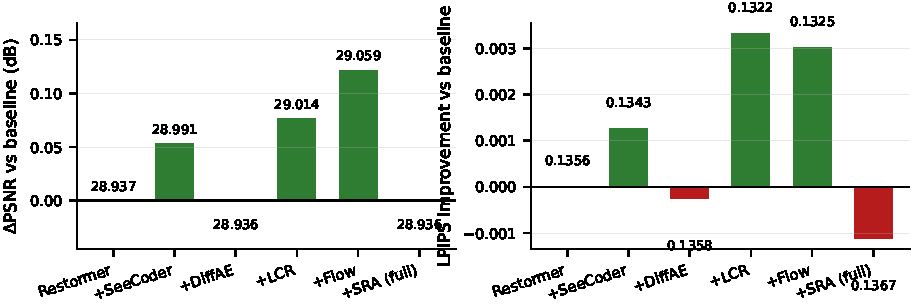
\includegraphics[width=\textwidth]{fig_ablation.pdf}
\caption{Per-module effect relative to the baseline, all 1111 test images.
Left: $\Delta$PSNR (higher better). Right: LPIPS improvement (higher better;
LPIPS itself is lower-better). Absolute values are printed above each bar.
DiffAE (C) and SRA (F) are indistinguishable from the baseline on PSNR, and SRA
degrades LPIPS significantly.}
\label{fig:ablation}
\end{figure*}

\section{Results}
\label{sec:results}

\subsection{Main ablation}
\label{sec:ablationresults}

Table~\ref{tab:main} reports all six configurations and Fig.~\ref{fig:ablation}
visualizes the per-module effect. Every arm completed its full 60-epoch cosine
schedule with the learning rate reaching $\eta_{\min}$, so every row is
admissible and no cell is estimated.

\begin{table}[t]
\caption{Ablation ladder on 1111 GoPro test images. $\Delta$ is the
\emph{paired per-image} mean PSNR difference from the baseline, with a 95\%
confidence interval over test images and a Wilcoxon signed-rank $p$.
Best per column in \bs{bold}.}
\label{tab:main}
\centering
\footnotesize
\setlength{\tabcolsep}{3.1pt}
\begin{tabular}{@{}llcccc@{}}
\toprule
& Configuration & PSNR & SSIM & LPIPS & Params \\
\midrule
A & Restormer                & 28.937 & 0.8661 & 0.1356 & 26.1M \\
B & \;+SeeCoder              & 28.991 & 0.8675 & 0.1343 & 26.6M \\
C & \;+DiffAE                & 28.936 & 0.8668 & 0.1358 & 28.0M \\
D & \;+LCR                   & 29.014 & 0.8683 & \bs{0.1322} & 33.1M \\
E & \;+Rectified flow        & \bs{29.059} & \bs{0.8694} & 0.1325 & 37.2M \\
F & \;+SRA (full SRRT)       & 28.936 & 0.8667 & 0.1367 & 37.2M \\
\midrule
\multicolumn{6}{@{}l}{\emph{Paired per-image $\Delta$PSNR vs.\ A}}\\
B & $+0.054$ & \multicolumn{2}{l}{$[+0.033,+0.074]$} & 675/436 & $p\!=\!8.5\mathrm{e}{-12}$ \\
C & $-0.001$ & \multicolumn{2}{l}{$[-0.020,+0.018]$} & 574/537 & $p\!=\!0.69$ \\
D & $+0.077$ & \multicolumn{2}{l}{$[+0.058,+0.095]$} & 678/433 & $p\!=\!8.7\mathrm{e}{-18}$ \\
E & $\bs{+0.122}$ & \multicolumn{2}{l}{$[+0.102,+0.142]$} & \bs{756/355} & $p\!=\!1.8\mathrm{e}{-38}$ \\
F & $-0.001$ & \multicolumn{2}{l}{$[-0.023,+0.021]$} & 550/561 & $p\!=\!0.51$ \\
\bottomrule
\end{tabular}
\end{table}

Three results stand out.

\bs{Rectified flow is the strongest module.} E improves on the baseline by
$+0.122$~dB, wins on 756 of 1111 images, and its confidence interval excludes
zero by a wide margin ($p=1.8\times10^{-38}$, Cohen's $d=0.353$). It is also
best on SSIM. Fig.~\ref{fig:qual} shows where this manifests: recovered
high-frequency structure on fence railings, vehicle edges and text-like detail.

\bs{The damage-aware encoder does nothing measurable.} C is
indistinguishable from the baseline on every metric ($p=0.69$, 574 wins to 537
losses---almost exactly chance). It adds 1.9M parameters for no effect. This is
consistent with our stated caveat that DiffAE is not shown to isolate
degradation; here it does not appear to represent anything the backbone was not
already using.

\bs{SRA cancels the accumulated gain.} E$\rightarrow$F is a pure SRA ablation,
and it removes the entire $+0.122$~dB, returning to baseline ($p=0.51$). On
LPIPS it is actively harmful ($+0.00112$, $p=9.8\times10^{-4}$). The module
that completes the architecture is the one that should be removed from it.

Fig.~\ref{fig:convergence} shows the arms are visually indistinguishable during
most of training and separate only in the final annealed epochs, which is why
the schedule-matching requirement of Section~\ref{sec:setup} matters: a run
stopped early would land anywhere in the bundle.

\begin{figure}[t]
\centering
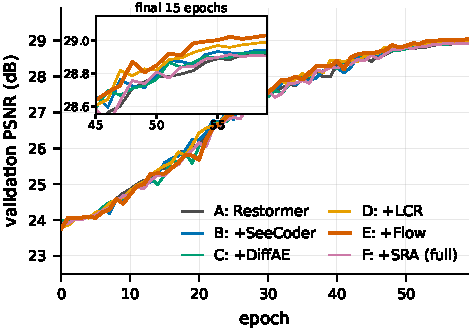
\includegraphics[width=\columnwidth]{fig_convergence.pdf}
\caption{Validation PSNR across all six arms. The arms are indistinguishable
for most of training; the inset over the final 15 epochs is where the ablation
becomes legible.}
\label{fig:convergence}
\end{figure}

\subsection{Admissibility}
\label{sec:admis}
A run enters Table~\ref{tab:main} only if it completed the full schedule with
the learning rate annealed to $\eta_{\min}$. This rule is not cosmetic. An
earlier SeeCoder run stopped at epoch 40 of 60 with the learning rate still at
$4.63\times10^{-5}$ and scored 28.496~dB---which, reported naively, would have
shown SeeCoder \emph{costing} 0.44~dB. Trained to completion the same
configuration scores 28.991~dB, a small but significant \emph{gain}. The
deficit was entirely an artifact of training length. We therefore discard
partial runs rather than report them with a caveat.

\subsection{Failure analysis of the rectified-flow integration}
\label{sec:flowfailure}

Our first flow configuration did not merely score poorly: it diverged. It fell
from 24.098~dB at epoch 5 to 14.527~dB at epoch 6 and reached 6.606~dB by epoch
9, while D---identical but for the flow module---climbed monotonically over the
same epochs (Fig.~\ref{fig:divergence}). Two independent defects were isolated,
each by a single-variable experiment.

\bs{Defect 1: the regression target was trainable.} The velocity target
$v^\star=z_1-z_0$ in \eqref{eq:velocity} was formed with $z_1$ still attached
to the graph. Because $z_1$ is produced by the \emph{shared restoration
encoder}, $\mathcal{L}_{\text{flow}}$ could be reduced by moving $z_1$ toward
$z_0$---by degrading the encoder the restoration path depends on---which is an
easier descent direction than learning $v_\theta$. It preferentially did so:
the flow loss deposited gradient of norm $4.23\times10^{-2}$ on the backbone
against $1.971\times10^{-2}$ on the velocity network it was meant to train. The
flow loss fell $31\times$ while PSNR fell 10~dB. Detaching $z_1$, as in
\eqref{eq:flow}, removes the degenerate minimum.

\bs{Defect 2: train/inference latent mismatch.} During training the backbone
was injected with the supervised endpoint $z_1$; at inference it receives the
ODE solution $\hat{z}_1$. The model learned to rely on an encoding of the
ground truth unavailable at test time. Measured on one checkpoint, injecting
the ground-truth latent gave 24.819~dB against 18.946~dB for the ODE
latent---a 5.874~dB gap between what training optimized and what inference
could deliver. Injecting $z_0$ during training, with the ODE solution used only
at inference, removes the asymmetry.

With both corrected, the configuration trains stably
(Fig.~\ref{fig:divergence}) and becomes the best arm in Table~\ref{tab:main}.
We regard the general lesson as transferable: \emph{an auxiliary loss whose
target is produced by a shared trainable component has a degenerate solution},
and a falling auxiliary loss alongside a falling task metric should be read as
a symptom rather than a curiosity.

\begin{figure}[t]
\centering
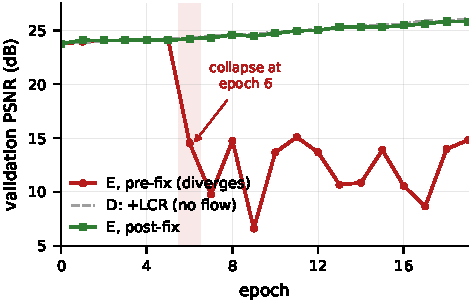
\includegraphics[width=\columnwidth]{fig_divergence.pdf}
\caption{The rectified-flow configuration before and after the two fixes of
Section~\ref{sec:flowfailure}, with D (identical but for the flow module) as
reference. Pre-fix, training collapses at epoch 6 and never recovers.}
\label{fig:divergence}
\end{figure}

\subsection{Computational cost}
Inference at $256\times256$ averages 0.218~s/image for the baseline and
0.424~s/image for E, whose ODE integration uses 20 Euler steps---roughly a
$1.9\times$ cost for $+0.122$~dB. Peak evaluation memory is 6.8~GB for A and
6.9~GB for E. Training one arm takes 6--8~h on the target GPU. GFLOPs are not
reported: neither \texttt{thop} nor \texttt{fvcore} was available in the
environment, and we decline to estimate them.

%=====================================================================
\section{Discussion and Limitations}
\label{sec:limitations}

\bs{Single seed per arm.} This is the binding limitation. The confidence
intervals in Table~\ref{tab:main} are over \emph{test images} for one fixed
pair of checkpoints. They answer ``would this difference survive a different
sample of GoPro-like images,'' and for B, D and E the answer is emphatically
yes. They say nothing about whether it would survive retraining with a
different seed. A statistically significant per-image difference of 0.12~dB may
still be seed noise, and a seed-repeat study is the prerequisite for upgrading
these from measured differences to claims about the method.

\bs{Validation and test are the same split.} The validation loader reads the
GoPro test split, so checkpoint selection and reported metrics use the same
1111 images. Reported figures may be mildly optimistic through model selection.
A validation subset should be carved from the training split.

\bs{Training budget.} At 15{,}720 optimizer steps and a fixed 128~px crop, all
arms are far from the published Restormer budget, with no progressive
patch-size schedule. Benefits requiring longer training or larger crops would
not appear. Indicatively, an unmatched 200-epoch schedule of configuration E
reached 29.65~dB validation PSNR by epoch 88---a larger gain than any module
contributes---suggesting budget dominates architecture in this regime.

\bs{Protocol.} Evaluation uses $256\times256$ center crops, not the full images
used for published GoPro numbers, so absolute values are not directly
comparable to the literature. The \emph{relative} comparisons, which are the
subject of this paper, are unaffected since all arms share the protocol.

\bs{Untrained sub-block.} The DiffAE semantic head (131{,}584 parameters) is
computed every forward pass but does not enter the objective, inflating the
parameter counts of C--F.

\bs{Scope.} Only GoPro motion deblurring; loss weights are untuned defaults.

%=====================================================================
\section{Conclusion}

We trained SRRT's full six-rung ablation ladder to convergence under a matched
schedule. Rectified-flow latent transport is the one clearly beneficial module
($+0.122$~dB, $p=1.8\times10^{-38}$); LCR contributes a smaller gain and the
best LPIPS; the damage-aware encoder contributes nothing measurable; and
semantic refinement attention cancels the accumulated gain and should be
removed. With one training run per arm these remain measured differences, not
established properties of the method.

Two findings transfer beyond this architecture: \emph{a zero-output equivalence
test cannot establish that a module is integrated}, only a gradient-flow check
can; and \emph{an auxiliary objective whose regression target is produced by a
shared trainable component admits a degenerate solution}, which ours took,
costing 10~dB until the target was detached.

Future work: a seed-repeat study to calibrate run-to-run variance, a held-out
validation split, a larger training budget, and redesign of the two modules
shown here to contribute nothing.

%=====================================================================
\begin{thebibliography}{00}
\footnotesize

\bibitem{restormer} S.~W. Zamir, A.~Arora, S.~Khan, M.~Hayat, F.~S. Khan, and
M.-H. Yang, ``Restormer: Efficient transformer for high-resolution image
restoration,'' in \emph{Proc. IEEE/CVF CVPR}, 2022, pp.~5728--5739.

\bibitem{swinir} J.~Liang, J.~Cao, G.~Sun, K.~Zhang, L.~Van Gool, and
R.~Timofte, ``SwinIR: Image restoration using Swin transformer,'' in
\emph{Proc. IEEE/CVF ICCV Workshops}, 2021, pp.~1833--1844.

\bibitem{uformer} Z.~Wang, X.~Cun, J.~Bao, W.~Zhou, J.~Liu, and H.~Li,
``Uformer: A general U-shaped transformer for image restoration,'' in
\emph{Proc. IEEE/CVF CVPR}, 2022, pp.~17683--17693.

\bibitem{nafnet} L.~Chen, X.~Chu, X.~Zhang, and J.~Sun, ``Simple baselines for
image restoration,'' in \emph{Proc. ECCV}, 2022, pp.~17--33.

\bibitem{gopro} S.~Nah, T.~H. Kim, and K.~M. Lee, ``Deep multi-scale
convolutional neural network for dynamic scene deblurring,'' in \emph{Proc.
IEEE CVPR}, 2017, pp.~3883--3891.

\bibitem{seecoder} X.~Xu, J.~Guo, Z.~Wang, G.~Huang, I.~Essa, and H.~Shi,
``Prompt-free diffusion: Taking ``text'' out of text-to-image diffusion
models,'' in \emph{Proc. IEEE/CVF CVPR}, 2024.

\bibitem{diffae} K.~Preechakul, N.~Chatthee, S.~Wizadwongsa, and
S.~Suwajanakorn, ``Diffusion autoencoders: Toward a meaningful and decodable
representation,'' in \emph{Proc. IEEE/CVF CVPR}, 2022, pp.~10619--10629.

\bibitem{rectifiedflow} X.~Liu, C.~Gong, and Q.~Liu, ``Flow straight and fast:
Learning to generate and transfer data with rectified flow,'' in \emph{Proc.
ICLR}, 2023.

\bibitem{ssim} Z.~Wang, A.~C. Bovik, H.~R. Sheikh, and E.~P. Simoncelli,
``Image quality assessment: From error visibility to structural similarity,''
\emph{IEEE Trans. Image Process.}, vol.~13, no.~4, pp.~600--612, 2004.

\bibitem{lpips} R.~Zhang, P.~Isola, A.~A. Efros, E.~Shechtman, and O.~Wang,
``The unreasonable effectiveness of deep features as a perceptual metric,'' in
\emph{Proc. IEEE/CVF CVPR}, 2018, pp.~586--595.

\bibitem{vgg} K.~Simonyan and A.~Zisserman, ``Very deep convolutional networks
for large-scale image recognition,'' in \emph{Proc. ICLR}, 2015.

\bibitem{adamw} I.~Loshchilov and F.~Hutter, ``Decoupled weight decay
regularization,'' in \emph{Proc. ICLR}, 2019.

\bibitem{sgdr} I.~Loshchilov and F.~Hutter, ``SGDR: Stochastic gradient descent
with warm restarts,'' in \emph{Proc. ICLR}, 2017.

\bibitem{amp} P.~Micikevicius \emph{et al.}, ``Mixed precision training,'' in
\emph{Proc. ICLR}, 2018.

\end{thebibliography}

\end{document}
